\documentclass[11pt,a4paper]{article}
\usepackage[utf8]{inputenc}
\usepackage[T1]{fontenc}
\usepackage{lmodern,microtype}
\usepackage[margin=2.4cm]{geometry}
\usepackage{booktabs,longtable,tabularx,array,multirow,pdflscape}
\usepackage{amsmath,amssymb}
\usepackage{tikz,pgfplots}
\pgfplotsset{compat=1.16}
\usetikzlibrary{positioning,arrows.meta,shapes.geometric}
\usepackage[authoryear,round]{natbib}
\usepackage[hidelinks]{hyperref}
\usepackage{xcolor,caption,setspace,graphicx}
\captionsetup{font=small,labelfont=bf}
\setlength{\parskip}{4pt}
\newcommand{\Npriorrev}{25}
\newcommand{\Nqueries}{70}
\newcommand{\Nretrieved}{7{,}000}
\newcommand{\Ndups}{4{,}763}
\newcommand{\Nunique}{2{,}237}
\newcommand{\Nother}{6}
\newcommand{\Nothernew}{4}
\newcommand{\Notherreinst}{2}
\newcommand{\Nscreened}{2{,}241}
\newcommand{\Nautoexcl}{2{,}145}
\newcommand{\Nassessed}{98}
\newcommand{\Nexclelig}{56}
\newcommand{\Nincluded}{41}
\newcommand{\NnF}{16}
\newcommand{\NnD}{11}
\newcommand{\NnS}{14}
\newcommand{\Nnabs}{33}
\newcommand{\Nnnoabs}{8}
\newcommand{\Nenotq}{33}
\newcommand{\Negrowth}{9}
\newcommand{\Negeo}{5}
\newcommand{\Nelang}{2}
\newcommand{\Neundet}{3}
\newcommand{\Neoper}{4}
\newcommand{\Nftsought}{42}
\newcommand{\Nftretr}{21}
\newcommand{\Nftnotret}{21}
\newcommand{\Nftexcl}{1}
\newcommand{\Nftconf}{20}
\newcommand{\Nabsonly}{21}
\newcommand{\Ndupsall}{4{,}765}
\newcommand{\Nautonet}{2{,}143}
\newcommand{\Nidentified}{7{,}006}
\newcommand{\Nsaudiall}{12}
\newcommand{\NsaudiF}{4}
\newcommand{\Nturk}{10}
\newcommand{\NFsust}{1}
\newcommand{\NnonFsust}{17}
\newcommand{\NnonFnosust}{8}
\newcommand{\NFnosust}{15}
\newcommand{\NFabs}{12}
\newcommand{\NFbench}{11}
\newcommand{\NFfuture}{4}
\newcommand{\NFmetric}{7}
\newcommand{\NFm}{6}
\newcommand{\NFc}{4}
\newcommand{\NFh}{5}
\newcommand{\NFg}{1}
\newcommand{\NnonFfut}{1}
\newcommand{\NnonFecon}{25}
\newcommand{\NnonFn}{25}
\newcommand{\Nprerecent}{4}
\newcommand{\Nyrecent}{37}
\newcommand{\Nyvrecent}{16}
\newcommand{\NSenv}{12}

\newcommand{\tbd}{\textcolor{red}{[to be completed]}}

\title{Forecasting and Sustainability in Middle Eastern Tourism, with Emphasis on Saudi Arabia:\\ A PRISMA~2020 Systematic Review of the Empirical Literature, 2015--2026}
\author{[Author name(s) and affiliation(s) --- to be completed]\\ \small Corresponding author: [e-mail]}
\date{Search conducted 5 October 2026}

\begin{document}
\maketitle

\begin{abstract}
\noindent\textbf{Background.} Tourism is a diversification pillar for Gulf economies, and Saudi Arabia in particular, yet it is unclear whether the empirical literature that forecasts tourism and the literature that studies its sustainability inform one another.
\textbf{Objectives.} To map and synthesise empirical studies of (A) tourism or hospitality forecasting, (B) tourism-demand modelling, and (C) quantitative tourism--sustainability analysis in Saudi Arabia and the wider Middle East, and to identify evidence gaps.
\textbf{Data sources.} Crossref REST API (journal articles, 2015--2026; \Nqueries{} queries; \Nretrieved{} records, \Nunique{} unique), plus targeted title searches seeded by web-search leads.
\textbf{Eligibility and appraisal.} Peer-reviewed quantitative studies in English set in the Middle East (MENA, GCC, T\"urkiye, Iran, Israel). Screening was by a single reviewer (an AI agent) at title/abstract/metadata level; full texts were not accessible. Quality was assessed with a six-item reporting-transparency screen, not a formal risk-of-bias tool.
\textbf{Results.} \Nincluded{} studies were included (\NnF{} forecasting, \NnD{} demand-modelling, \NnS{} sustainability-nexus); \Nyrecent{} appeared from 2020 onward. Saudi Arabia was the setting of \Nsaudiall{} studies but only \NsaudiF{} forecasting studies. Of \NnF{} forecasting studies, only \NFsust{} addressed sustainability; all \NnonFn{} non-forecasting studies used econometric or statistical designs, only \NnonFfut{} projected outcomes forward (climate-scenario simulation), and none evaluated out-of-sample forecast accuracy. Within the retrieved corpus the two literatures are therefore largely disconnected.
\textbf{Conclusions.} Forecasts are rarely linked to environmental or capacity outcomes, and sustainability analyses are mostly ex post. We outline a capacity-aware forecasting agenda. Findings are bounded by retrieval caps, abstract-level coding and single-reviewer screening, and must be confirmed against full texts before submission.
\textbf{Registration.} Not registered.
\end{abstract}
\noindent\textbf{Keywords:} tourism demand forecasting; sustainability; Saudi Arabia; Vision 2030; Middle East; machine learning; PRISMA 2020

\section{Introduction}
Tourism is central to the economic diversification plans of Gulf states. Saudi studies frame tourism research around Vision 2030 and diversification away from oil dependency \citep{Alamoudi2020,Abuhulaibah2026}, and recent work links tourism growth to climate and environmental outcomes in the Kingdom \citep{Chouari2025,Alfehaid2026,Raihan2025}. Two methodological traditions are relevant. The first is tourism demand forecasting, which has been reviewed repeatedly in global terms \citep{Song2019,Peng2014,Jiao2019} and has moved from time-series and econometric models toward machine learning, deep learning and internet-search data \citep{Law2019,Zhang2020}. General forecasting competitions have emphasised out-of-sample evaluation against strong benchmarks \citep{Makridakis2020,Makridakis2022}. The second tradition is the quantitative analysis of tourism's economic, social and environmental consequences, typically through cointegration and panel designs.

Saudi-focused work has examined tourism's contribution to Vision 2030 and SDG~8 \citep{Saudi2024sdg}, but within the sources retrieved here we did not identify a PRISMA-guided review that examines \emph{forecasting} and \emph{sustainability} evidence together for Saudi Arabia and the Middle East. This matters because forecasts are used to plan capacity and investment, whereas sustainability outcomes depend on that capacity. If the two literatures do not meet, forecasts may be accurate yet blind to environmental limits, and sustainability analyses may be rigorous yet unable to anticipate future pressure.

\paragraph{Objectives.} Following PRISMA~2020 \citep{Page2021,Page2021ee}, we ask: \textbf{RQ1} What forecasting, demand-modelling and tourism--sustainability studies exist for Saudi Arabia and the Middle East, and what are their settings and methods? \textbf{RQ2} How rigorously are forecasting studies evaluated, as visible in their reporting? \textbf{RQ3} To what extent do forecasting studies incorporate sustainability, and do sustainability studies produce forecasts? \textbf{RQ4} What research agenda follows?

\paragraph{Contributions relative to prior reviews.} Section~\ref{sec:prior} compares this review with the closest of \Npriorrev{} prior reviews whose bibliographic records were verified in Crossref. Against that set, the review contributes: (i) a joint, PRISMA-structured map of \emph{forecasting} and \emph{quantitative sustainability} evidence for Saudi Arabia and the Middle East, a scope that, among the reviews we located, is covered only in parts (global forecasting reviews; global tourism--carbon and carrying-capacity reviews; regional reviews of GCC or Saudi tourism without a forecasting lens); (ii) a cross-classification showing that the two literatures are largely disconnected in this region, together with a typology of the \emph{direction} of the tourism--environment links that are studied; (iii) a regional comparison of these findings with the global reviews; and (iv) a research agenda positioned against the existing carrying-capacity early-warning literature. Contribution (i) is a scope contribution, and (ii)--(iii) are synthesis contributions; we do not claim methodological novelty in review procedure.


\section{Literature Background and Related Reviews}\label{sec:prior}
We searched Crossref for prior reviews with 24 logged queries (review, bibliometric, meta-analysis and scoping-review terms combined with forecasting, sustainability, carbon, carrying capacity, Saudi Arabia, GCC and Middle East; \texttt{prior/prior\_search\_log.json}) and checked additional regional reviews by web search. This identified \Npriorrev{} closely related reviews; all are listed with their open-access status in the repository (\texttt{prior/}, \texttt{data/oa\_status.json}). To keep the reference list mostly open access, Table~\ref{tab:prior} shows the open-access reviews together with the three closed-access reviews that the novelty argument depends on \citep{Jiao2019,Sun2022,Saleh2021}. Omitting the other closed-access reviews does not change the conclusions below: none of them, judged from abstract or title, covers forecasting and sustainability together for this region. Scope is coded from the Crossref abstract where one is deposited and otherwise from the title; two entries rely on web-search snippets and are marked.

\emph{Global forecasting reviews} synthesise models, data sources and accuracy \citep{Peng2014,Jiao2019,Song2019,Zhang2020km,Dowlut2023,Wu2024,Henriques2024}. Where abstracts are available, none indicates a regional focus on the Middle East or a sustainability dimension.

\emph{Tourism--sustainability reviews} address carbon emissions \citep{Sun2022}, automation for sustainability \citep{Majid2023} and carrying capacity \citep{Long2022,Ajuhari2023}. The closest is \citet{Sun2022}, a systematic review of econometric tourism--emission studies, which overlaps our Theme~S in method and outcome but is global. The carrying-capacity reviews are the only ones that connect sustainability to forecasting: \citet{Long2022} call for improved dynamic forecasting and early warning of tourism environmental carrying capacity, and primary studies already forecast early-warning indices \citep[e.g.][]{Ye2020}.

\emph{Regional reviews} cover GCC tourism research \citep{Saleh2021}, Saudi tourism and SDG~8 \citep{Saudi2024sdg} and ESG in Saudi hotels \citep{Alhejaili2025}. The closest is \citet{Saleh2021}, a PRISMA review of 23 GCC tourism studies, which found most to focus on Dubai and on tourism planning; its abstract does not indicate coverage of forecasting.

\paragraph{Closest prior work and difference.} The two reviews most dangerous to our novelty claim are \citet{Saleh2021} (same region and reporting standard) and \citet{Sun2022} (same sustainability outcome and study designs). This review differs from both in jointly coding forecasting and sustainability studies and analysing their connection, in extending the region to the Middle East with a Saudi focus, and in covering 2015--2026, including the post-2021 growth in Saudi studies. It is narrower than both in one respect, as it rests on abstract-level coding (Section~\ref{sec:limits}). We therefore state its novelty conservatively: among the reviews we located, none jointly synthesises forecasting and quantitative sustainability evidence for this region.

\begin{landscape}
\begin{table}[p]\centering\scriptsize
\caption{Closest prior reviews compared with this review (open-access reviews plus the closed-access reviews essential to the comparison). F = forecasting; S = sustainability; F$\leftrightarrow$S = analyses links between forecasting and sustainability. \checkmark\ = indicated; -- = not indicated; ``title'' = abstract not deposited in Crossref, scope coded from the title only; ``snippet'' = scope from web-search snippet (unverified). Access from Unpaywall (gold, hybrid, green, bronze = open access).}\label{tab:prior}
\begin{tabular}{@{}p{3.8cm}p{3.2cm}p{2.8cm}p{2.4cm}cccp{2.4cm}p{1.6cm}p{1.2cm}@{}}
\toprule
Review & Type, sample & Coverage & Region & F & S & F$\leftrightarrow$S & Scope coded from & Access\\
\midrule
\multicolumn{9}{@{}l}{\textit{Global forecasting reviews}}\\
\citet{Peng2014} & Meta-analysis & n/r & Global & \checkmark & -- & -- & title & green\\
\citet{Jiao2019} & Review, 72 studies & 2008--2017 & Global & \checkmark & -- & -- & abstract & closed\\
\citet{Song2019} & Curated review & n/r & Global & \checkmark & -- & -- & title & bronze\\
\citet{Zhang2020km} & Knowledge mapping & n/r & Global & \checkmark & -- & -- & title & green\\
\citet{Dowlut2023} & SLR (deep learning) & resort hotels & Global & \checkmark & -- & -- & title & gold\\
\citet{Wu2024} & Systematic (big data) & n/r & Global & \checkmark & -- & -- & abstract & hybrid\\
\citet{Henriques2024} & PRISMA SLR, 20 & Scopus, WoS & Global & \checkmark & -- & -- & abstract & gold\\
\multicolumn{9}{@{}l}{\textit{Tourism--sustainability reviews}}\\
\citet{Sun2022} & Systematic, 81 econometric studies & 2013--2021 & Global & -- & \checkmark & partial (decarbonisation scenarios) & snippet & closed\\
\citet{Majid2023} & Systematic & automation & Global & -- & \checkmark & -- & title & hybrid\\
\citet{Long2022} & Bibliometric, 297 & carrying capacity & Global & partial & \checkmark & calls for forecasting/early warning & abstract & gold\\
\citet{Ajuhari2023} & SLR, 100 & carrying-capacity methods & Global & -- & \checkmark & -- & abstract & gold\\
\multicolumn{9}{@{}l}{\textit{Regional reviews}}\\
\citet{Saleh2021} & PRISMA SR, 23 & GCC tourism & GCC & -- & partial (impacts) & -- & abstract & closed\\
\citet{Saudi2024sdg} & SLR & Vision 2030, SDG 8 & Saudi Arabia & -- & \checkmark & -- & snippet & hybrid\\
\citet{Alhejaili2025} & Literature review & ESG, 2020--2024 & Saudi hotels & -- & \checkmark & -- & abstract & gold\\
\midrule
\textbf{This review} & PRISMA SR, \Nincluded{} studies & 2015--2026, Crossref & Middle East, Saudi focus & \checkmark & \checkmark & \checkmark\ (cross-classified) & abstract & --\\
\bottomrule
\end{tabular}
\end{table}
\end{landscape}

\section{Methodology}
The review follows the PRISMA~2020 statement; the completed checklist, with honest status per item, is in Appendix~A. Deviations are reported explicitly below and in Section~\ref{sec:limits}.

\subsection{Review Protocol and Registration}
No protocol was registered. The inclusion criteria, search design and coding scheme were fixed before the eligibility stage and are archived with the code and data (Appendix~D). Registration on a general registry such as OSF is recommended before journal submission.

\subsection{Information Sources}
The primary source was the Crossref REST API (accessed 5 October 2026), filtered to journal articles published 1~January 2015 to 31~December 2026. Crossref was chosen because it was the only bibliographic index reachable from the execution environment; Scopus, Web of Science and Google Scholar were not accessible. Four earlier web-search screening passes (\emph{search snippets only}) produced candidate leads. These leads were not counted as identified records; they seeded targeted Crossref title searches (``other methods''), and every record that was retained had its metadata re-verified by DOI lookup in Crossref. Publisher full texts could not be retrieved because the environment's network policy returned errors for publisher and DOI-resolver hosts (Section~\ref{sec:limits}).

\subsection{Search Strategy}
We ran \Nqueries{} queries using the \texttt{query.bibliographic} parameter with \texttt{rows}=100: eight concept strings (e.g. ``tourism demand forecasting'', ``tourism CO2 emissions'', ``sustainable tourism modelling'') crossed with four regional terms (Saudi Arabia, Middle East, GCC, Hajj/Umrah), plus ``tourism demand forecasting'' and ``tourism sustainability'' for 19 additional location terms (Appendix~C). Each query returned its 100 top-ranked records, so retrieval is capped and not exhaustive (Crossref's reported totals count fuzzy matches across all works and are not counts of relevant records) (Section~\ref{sec:limits}). The full list, dates and reported totals are in Appendix~C and \texttt{data/search\_log.json}. PRISMA-S was not formally applied; the limits of relying on a single index are discussed by \citet{Gusenbauer2020}.

Table~\ref{tab:strings} summarises the strategy.

\begin{table}[t]\centering\small
\caption{Search strategy: databases, search strings and filters (full query log in Appendix~C).}\label{tab:strings}
\begin{tabularx}{\linewidth}{@{}p{3.1cm}X@{}}
\toprule
Element & Specification\\
\midrule
Database & Crossref REST API (\texttt{query.bibliographic}); accessed 5 October 2026\\
Concept block (8 strings) & ``tourism demand forecasting'', ``tourist arrivals forecasting'', ``tourism forecasting machine learning'', ``tourism forecasting deep learning'', ``hotel occupancy forecasting'', ``tourism sustainability prediction'', ``tourism CO2 emissions'', ``sustainable tourism modelling''\\
Location block 1 (crossed with concepts) & Saudi Arabia; Middle East; GCC; Hajj Umrah\\
Location block 2 (with ``tourism demand forecasting'' and ``tourism sustainability'') & Gulf Cooperation Council; GCC; Middle East; MENA; Dubai; UAE; United Arab Emirates; Qatar; Oman; Bahrain; Kuwait; Jordan; Egypt; Turkey; Iran; Morocco; Tunisia; Lebanon; Israel\\
Filters & Document type = journal article; publication date 1 January 2015 -- 31 December 2026; top 100 records per query\\
Other methods & Targeted Crossref title searches seeded by web-search leads; DOI verification of every retained record\\
\bottomrule
\end{tabularx}
\end{table}

\subsection{Inclusion and Exclusion Criteria}
Studies were eligible if they: (i) were peer-reviewed journal articles, 2015--2026; (ii) were reported in English; (iii) were set in the Middle East, defined here as Saudi Arabia, the other GCC states, MENA countries, T\"urkiye, Iran, Iraq and Israel (multi-country panels were eligible when Middle Eastern units were analysed); and (iv) were quantitative empirical studies falling under one of three themes: \textbf{F} -- forecasting of tourism or hospitality outcomes (arrivals, demand, spending, revenue, hotel price or occupancy); \textbf{D} -- econometric or statistical modelling of tourism demand or outcomes without a forecasting objective; \textbf{S} -- quantitative analysis of tourism together with a sustainability dimension (environmental, social or economic-sustainability variables). Excluded were studies that examined only the tourism--economic-growth nexus without a demand or sustainability outcome, perception or structural-equation surveys, qualitative or conceptual work, operational prediction such as crowd control or clinical outcomes during pilgrimage, non-journal records, and records whose region or tourism link could not be determined from the available metadata.

 The criteria are summarised in Table~\ref{tab:criteria}.

\begin{table}[t]\centering\small
\caption{Inclusion and exclusion criteria.}\label{tab:criteria}
\begin{tabularx}{\linewidth}{@{}p{2.6cm}XX@{}}
\toprule
Criterion & Inclusion & Exclusion\\
\midrule
Publication type & Peer-reviewed journal article & Conference proceedings, book chapters, theses, preprints\\
Period & 2015--2026 & Before 2015\\
Language & English & Other languages\\
Setting & Saudi Arabia, other GCC states, MENA, T\"urkiye, Iran, Iraq, Israel; multi-country panels with Middle Eastern units & No Middle Eastern unit analysed\\
Design & Quantitative empirical study & Perception or SEM surveys, qualitative, conceptual or review papers\\
Topic & F: forecasting a tourism or hospitality outcome; D: modelling tourism demand or outcomes; S: tourism with an environmental, social or economic-sustainability variable & Tourism--growth nexus only; crowd, health or operational prediction; non-tourism outcomes\\
Information & Region and tourism link determinable from metadata or abstract & Region or tourism link not determinable\\
\bottomrule
\end{tabularx}
\end{table}


\subsection{Study Selection}\label{sec:selection}
Selection had three stages. \emph{Stage 1} (automated): deduplication by DOI, then a rule-based filter requiring a tourism term, a Middle East location term and a forecasting or sustainability term in the title or abstract (\texttt{search/screen.py}). \emph{Stage 2} (automated): a method-term filter (forecast, predict, time series, ARDL, regression, machine learning and similar; \texttt{search/screen\_stage2.py}). \emph{Stage 3} (manual): title/abstract/metadata eligibility assessment of the remaining records, using the criteria above, with a reason recorded for every exclusion (Appendix~E). One reviewer, an AI agent, performed Stage~3; there was no independent duplicate screening. Because full texts were unavailable, ``reports assessed for eligibility'' in Figure~\ref{fig:prisma} means assessment of metadata and abstract, not full text.

\begin{figure}[t]
\centering
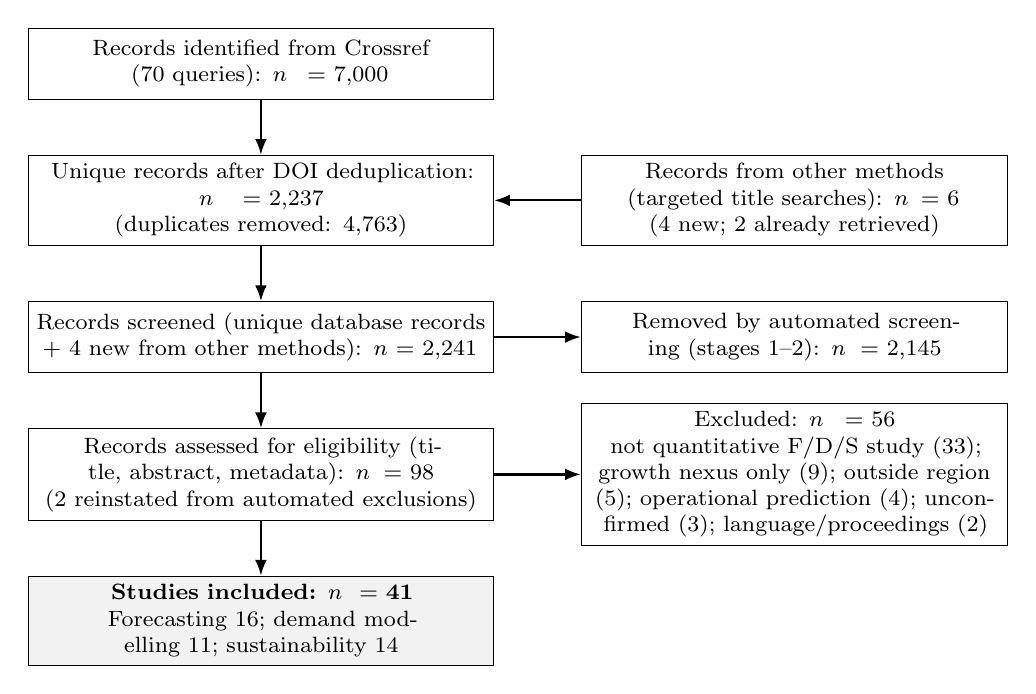
\begin{tikzpicture}[font=\footnotesize,node distance=7mm,
 box/.style={draw,rectangle,align=center,text width=5.7cm,minimum height=9mm,inner sep=3pt},
 side/.style={draw,rectangle,align=center,text width=5.2cm,minimum height=9mm,inner sep=3pt},
 lab/.style={draw,fill=gray!15,rotate=90,minimum width=2.2cm,align=center,font=\footnotesize\bfseries},
 arr/.style={-{Latex[length=2mm]},thick}]
\node[box] (id1) {Records identified from Crossref\\ (\Nqueries{} queries): $n=$ \Nretrieved{}};
\node[box,below=of id1] (id2) {Unique records after DOI deduplication:\\ $n=$ \Nunique{}\\ (duplicates removed: \Ndups{})};
\node[side,right=11mm of id2] (oth) {Records from other methods\\ (targeted title searches): $n=$ \Nother{}\\ (\Nothernew{} new; \Notherreinst{} already retrieved)};
\node[box,below=of id2] (scr) {Records screened (unique database records + \Nothernew{} new from other methods): $n=$ \Nscreened{}};
\node[side,right=11mm of scr] (ex1) {Removed by automated screening (stages 1--2): $n=$ \Nautoexcl{}};
\node[box,below=of scr] (ass) {Records assessed for eligibility (title, abstract, metadata): $n=$ \Nassessed{}\\ (\Notherreinst{} reinstated from automated exclusions)};
\node[side,right=11mm of ass] (ex2) {Excluded: $n=$ \Nexclelig{}\\ not quantitative F/D/S study (\Nenotq{}); growth nexus only (\Negrowth{}); outside region (\Negeo{}); operational prediction (\Neoper{}); unconfirmed (\Neundet{}); language/proceedings (\Nelang{})};
\node[box,below=of ass,fill=gray!10] (inc) {\textbf{Studies included: $n=$ \Nincluded{}}\\ Forecasting \NnF{}; demand modelling \NnD{}; sustainability \NnS{}};
\draw[arr](id1)--(id2); \draw[arr](id2)--(scr); \draw[arr](scr)--(ass); \draw[arr](ass)--(inc);
\draw[arr](scr)--(ex1); \draw[arr](ass)--(ex2); \draw[arr](oth.west)--(id2.east);
\end{tikzpicture}
\caption{PRISMA~2020 flow diagram. No full-text retrieval was possible, so eligibility was assessed on metadata and abstracts.}\label{fig:prisma}
\end{figure}


\subsection{Data Extraction}
The same reviewer coded each included study from the abstract and bibliographic record (\texttt{data/included.json}): theme; country; outcome; data period and frequency; method family (classical statistical or econometric, machine or deep learning, hybrid, ensemble or multi-family comparison, grey); presence of a benchmark comparison; reporting of an accuracy metric; presence of a forward projection; and sustainability dimension. Items not visible in the abstract were coded ``n/r'' and never inferred. Open-access status was recorded for every included study with Unpaywall (\texttt{data/oa\_status.json}): 31 of the \Nincluded{} are open access and 11 are closed access. Access did not influence eligibility, because excluding closed-access studies would bias a systematic review. For \Nnnoabs{} of the \Nincluded{} included records, Crossref held no abstract; these were coded from title and metadata only and are flagged in the tables.

The extraction form is shown in Table~\ref{tab:extraction}.

\begin{table}[t]\centering\small
\caption{Data extraction form (abstract-level; coding scheme in Appendix~B).}\label{tab:extraction}
\begin{tabularx}{\linewidth}{@{}p{3.6cm}X@{}}
\toprule
Item & Values\\
\midrule
Bibliographic & Authors, year, journal, volume, pages, DOI (Crossref); open-access status (Unpaywall)\\
Theme & F (forecasting), D (demand modelling), S (sustainability)\\
Setting & Country or multi-country panel\\
Outcome & e.g.\ arrivals, spending, revenue, hotel price or occupancy, CO$_2$, income equality\\
Data & Period and frequency\\
Method family & Classical; machine or deep learning; hybrid, ensemble or multi-family comparison; grey\\
Evaluation (F only) & Benchmark comparison; accuracy measure named; forward projection or scenario\\
Sustainability & Dimension stated (environmental, social, economic-sustainability, climate) or framing only\\
\bottomrule
\end{tabularx}
\end{table}

\subsection{Quality Appraisal}
A formal risk-of-bias tool for forecasting studies such as PROBAST \citep{Wolff2019} requires full-text information on participants, predictors and analysis, which was unavailable. We therefore applied a six-item \emph{reporting-transparency screen} to forecasting studies using abstract-visible information: data period and frequency stated; named benchmark comparison; accuracy metric reported; forward projection produced; sustainability link; and abstract available. This screen indicates reporting practice only; it is not a risk-of-bias judgment, and no study was excluded on this basis. Standard forecast-evaluation practice, namely out-of-sample accuracy measures and prediction intervals \citep{Hyndman2021fpp} and tests of predictive accuracy \citep{Diebold1995}, served as the reference for what a strong evaluation would report.

\subsection{Data Analysis}
Following the competing reviews, the analysis has three parts. (i) A descriptive analysis of publication years, journals, settings, method families and accuracy measures (Figures~\ref{fig:trend}--\ref{fig:measures}). (ii) A keyword co-occurrence analysis: because author keywords are not deposited in Crossref, we applied a controlled vocabulary of 28 terms (\texttt{search/make\_figures.py}) to titles and abstracts, retained terms occurring in at least three studies, linked terms co-occurring in at least two, and detected clusters by greedy modularity maximisation (Figure~\ref{fig:keywords}). (iii) A thematic synthesis by theme (F, D, S), followed by a cross-theme analysis. No meta-analysis or effect-size pooling was attempted because outcomes, horizons and metrics are heterogeneous and most accuracy values are not visible in abstracts. Reporting-bias and certainty-of-evidence assessments (PRISMA items 14, 15, 21, 22) were not performed.

\section{Results}
\subsection{Overview of the Included Studies}
The \Nqueries{} Crossref queries returned \Nretrieved{} records, of which \Ndups{} were duplicates, leaving \Nunique{} unique records. Four further records came from targeted searches and two others, found by those searches, had already been retrieved but removed by automated screening; \Nscreened{} records were therefore screened and \Nautoexcl{} were removed by the automated stages. Of \Nassessed{} records assessed at abstract level, \Nexclelig{} were excluded (Figure~\ref{fig:prisma}), leaving \Nincluded{} studies (Section~\ref{sec:selection}, Figure~\ref{fig:prisma}). Exclusion reasons were: not a quantitative forecasting, demand or sustainability study (\Nenotq{}); tourism--growth nexus only (\Negrowth{}); outside the Middle East (\Negeo{}); operational, crowd or health prediction (\Neoper{}); region or tourism link unconfirmed (\Neundet{}); and non-English or proceedings (\Nelang{}). The two records reinstated after automated exclusion show that the automated filters have imperfect recall (Section~\ref{sec:limits}).


\begin{figure}[t]\centering
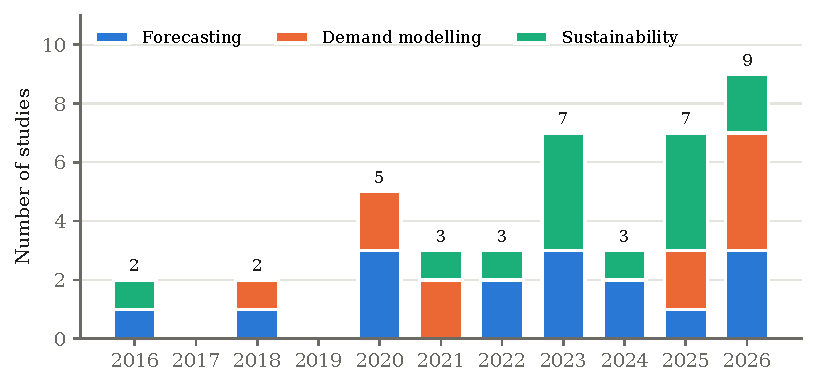
\includegraphics[width=\linewidth]{figs/fig_trend.pdf}
\caption{Year-wise distribution of the \Nincluded{} included studies by theme. Labels give annual totals.}\label{fig:trend}
\end{figure}

\begin{figure}[t]\centering
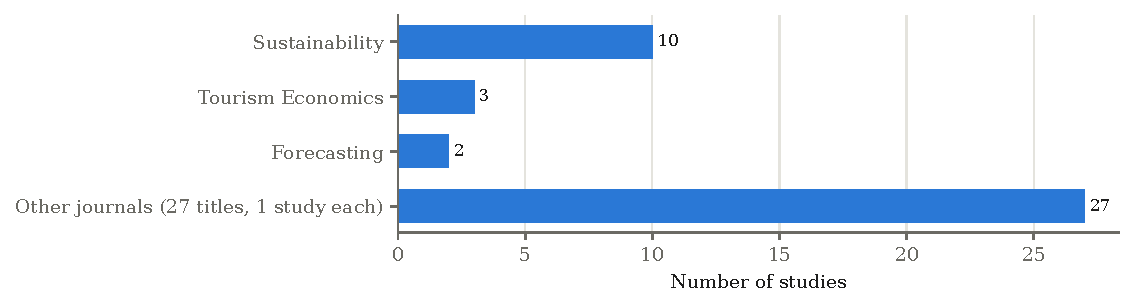
\includegraphics[width=\linewidth]{figs/fig_journals.pdf}
\caption{Journals publishing the included studies. Journals with a single included study are pooled.}\label{fig:journals}
\end{figure}

\begin{figure}[t]\centering
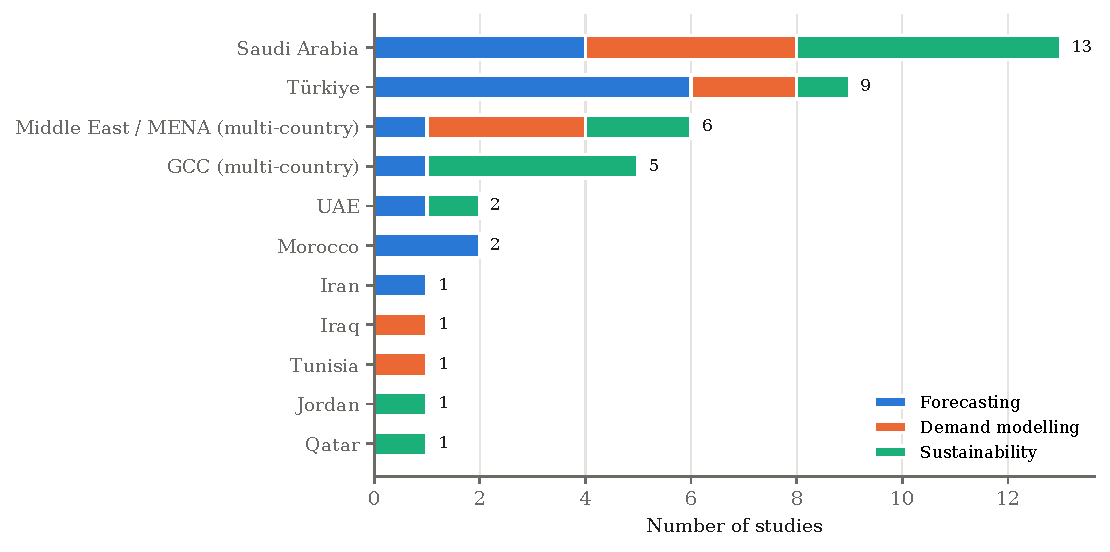
\includegraphics[width=\linewidth]{figs/fig_settings.pdf}
\caption{Study setting by theme. Multi-country panels are shown separately; the study covering Saudi Arabia, T\"urkiye and Italy is counted under Saudi Arabia.}\label{fig:settings}
\end{figure}

The \Nincluded{} included studies span 2016--2026; \Nyrecent{} appeared from 2020 and \Nyvrecent{} from 2025 (Figure~\ref{fig:trend}). They appeared in 30 journals; \emph{Sustainability} published 10, \emph{Tourism Economics} 3 and \emph{Forecasting} 2, and the remaining 27 appeared in different journals (Figure~\ref{fig:journals}). Saudi Arabia was the most frequent setting (13 studies), followed by T\"urkiye (9), multi-country Middle East or MENA panels (6) and GCC panels (5) (Figure~\ref{fig:settings}). Forecasting studies concentrate on T\"urkiye (6) and Saudi Arabia (4); sustainability studies on Saudi Arabia and GCC panels.

\subsection{Keyword Co-occurrence Analysis}
The co-occurrence network has 24 terms and 106 links (Figure~\ref{fig:keywords}). Modularity clustering separates two groups. The first (blue) combines forecasting, tourism demand, tourist arrivals, ARIMA/SARIMA, machine and deep learning, search data, seasonality, COVID-19 and T\"urkiye. The second (orange) combines sustainability, CO$_2$ emissions, energy, EKC, economic growth, ARDL/cointegration, causality, panel data, religious tourism, Vision 2030, GCC and Saudi Arabia. Only 23\% of co-occurrence weight crosses the two clusters, and the strongest bridges pass through \emph{tourist arrivals}, which sustainability studies use as an explanatory variable rather than as a forecast target. The term \emph{forecasting} co-occurs with \emph{sustainability} in only two studies and with CO$_2$, energy or EKC terms in fewer than two. The network thus anticipates the thematic finding in Section~\ref{sec:split}.

\begin{figure}[t]\centering
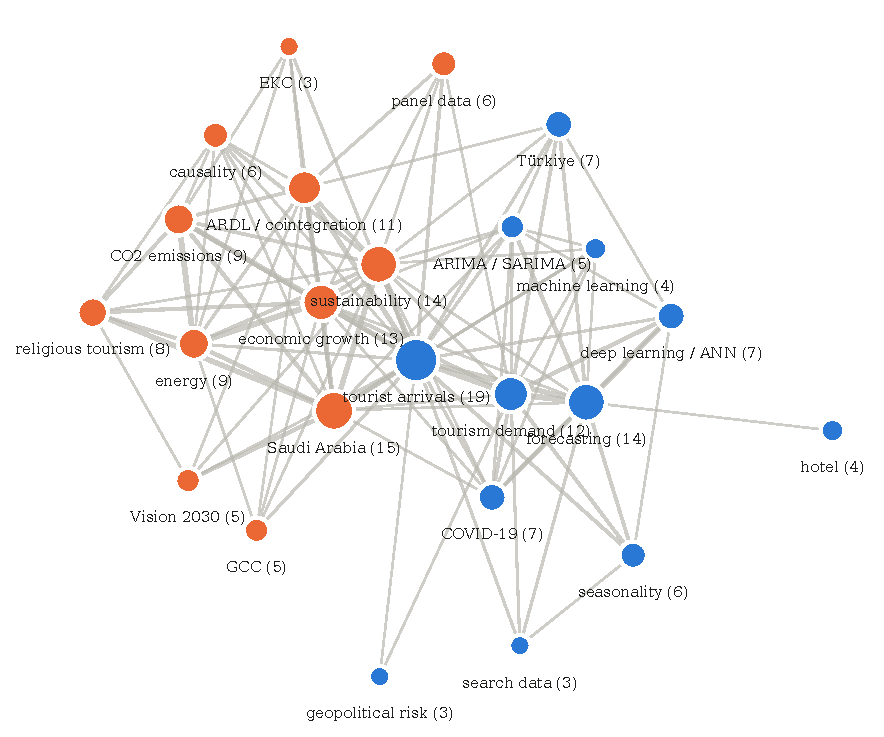
\includegraphics[width=0.95\linewidth]{figs/fig_keywords.pdf}
\caption{Keyword co-occurrence network of the included studies (controlled vocabulary applied to titles and abstracts). Node size reflects the number of studies containing the term (in brackets); line width reflects co-occurrence. Colours show the two modularity clusters: forecasting (blue) and sustainability--econometrics (orange).}\label{fig:keywords}
\end{figure}

\subsection{Theme 1: Forecasting Studies}
\NnF{} studies forecast a tourism or hospitality outcome (Table~\ref{tab:forecast}). By method family (Figure~\ref{fig:methods}), \NFm{} used machine or deep learning, \NFc{} classical models, \NFh{} hybrid or ensemble designs and \NFg{} grey model. Of the \NFabs{} studies whose abstracts were available, \NFbench{} compared several models or benchmarks, which is encouraging. \NFmetric{} abstracts named an accuracy metric, most often MAPE (5) and RMSE (3) (Figure~\ref{fig:measures}), but only \NFfuture{} produced a forward projection or scenario. Saudi forecasting evidence is thin: \NsaudiF{} studies, covering annual Umrah visitors to 2030 \citep{Alamoudi2020}, spending and ARIMA projections to 2030 \citep{Louati2024}, a machine-learning demand model with a geopolitical-instability proxy \citep{Zamzami2026}, and a machine-learning growth model whose abstract was unavailable \citep{Alsulami2026}. GCC hotel price forecasting with deep learning \citep{AlShehhi2020} and MENA hotel prices \citep{AlShehhi2018} are outside the arrivals-demand focus but within Theme F. Search-data forecasting of Dubai tourism \citep{Rashad2022} and Marrakech arrivals \citep{Laaroussi2023} indicate that internet-search predictors, studied globally \citep{Wu2024}, have reached the region.


\begin{figure}[t]\centering
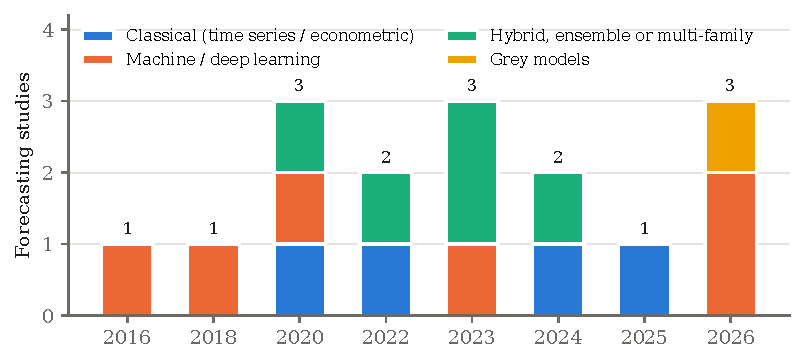
\includegraphics[width=\linewidth]{figs/fig_methods_year.pdf}
\caption{Forecasting studies by method family and publication year ($n=\NnF$).}\label{fig:methods}
\end{figure}

\begin{figure}[t]\centering
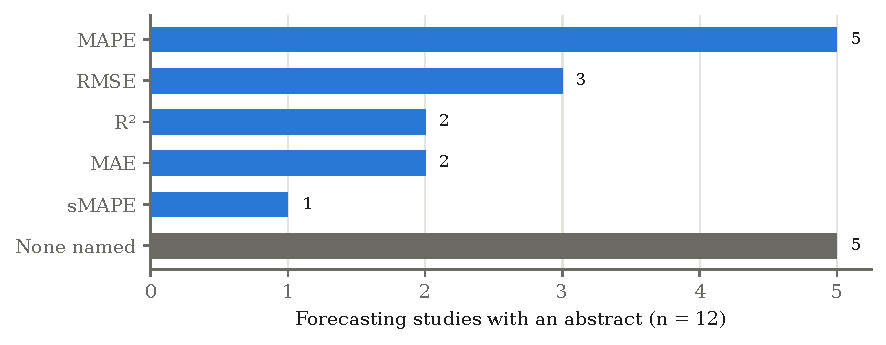
\includegraphics[width=\linewidth]{figs/fig_measures.pdf}
\caption{Accuracy measures named in the abstracts of forecasting studies. A study can name several measures.}\label{fig:measures}
\end{figure}

\begin{landscape}
\begin{table}[p]
\centering\small
\caption{Forecasting studies (Theme F). ``Benchmark'': named comparison of models or benchmarks in the abstract; ``n/r'': not reported or abstract unavailable. Coded from abstracts and metadata only.}\label{tab:forecast}
\begin{tabularx}{\linewidth}{@{}p{3.2cm}p{3.0cm}p{4.6cm}p{4.2cm}p{2.6cm}p{1.7cm}p{2.6cm}@{}}
\toprule
Study & Setting & Outcome & Data & Method family & Benchmark & Forward projection\\
\midrule
\citet{AlShehhi2020} & GCC cities & hotel room prices & n/r (abstract unavailable) & ML/DL & n/r & n/r \\
\citet{Ahmadian2026} & Iran & inbound tourist arrivals & 2020-2023 (small sample) & Grey & Yes & Yes (2024-26) \\
\citet{AlShehhi2018} & MENA cities & hotel prices & n/r (abstract unavailable) & ML/DL & n/r & n/r \\
\citet{Ouassou2022} & Morocco & regional tourist arrivals & annual, 1999-2018 & Hybrid/ensemble & Yes & No \\
\citet{Laaroussi2023} & Morocco (Marrakech) & tourist arrivals & monthly & Hybrid/ensemble & Yes & No \\
\citet{Louati2024} & Saudi Arabia & tourist spending; economic landscape & 2015-2021 & Hybrid/ensemble & Yes & Yes (2022-30) \\
\citet{Alsulami2026} & Saudi Arabia & tourism growth & n/r (abstract unavailable) & ML/DL & n/r & n/r \\
\citet{Zamzami2026} & Saudi Arabia & tourism demand (tourist numbers) & 2015-2024 & ML/DL & Yes & No \\
\citet{Alamoudi2020} & Saudi Arabia (Makkah) & international Umrah visitors & annual, 33 years & Classical & Yes & Yes (2020-30) \\
\citet{Cankurt2016} & T\"urkiye & tourism demand & n/r (abstract unavailable) & ML/DL & n/r & n/r \\
\citet{Cuhadar2020} & T\"urkiye & tourism revenues & n/r & Hybrid/ensemble & Yes & No \\
\citet{Tuncsiper2023} & T\"urkiye & tourist numbers; tourism revenue & monthly, 2008-2022 & ML/DL & No & No \\
\citet{Kayral2023} & T\"urkiye & tourist arrivals; tourism income & n/r & Hybrid/ensemble & Yes & Yes (scenarios) \\
\citet{Kurtulay2024} & T\"urkiye & international visitor demand & monthly, 2002-01 to 2023-08 & Classical & Yes & No \\
\citet{Bilek2025} & T\"urkiye & tourism demand & monthly, 2008-2024 & Classical & Yes & No \\
\citet{Rashad2022} & UAE (Dubai) & tourism demand (travel search data) & monthly, 2019-01 to 2022-04 & Classical & Yes & No \\
\bottomrule
\end{tabularx}

\end{table}
\end{landscape}

\subsection{Themes 2 and 3: Demand-Modelling and Sustainability Studies}
The remaining \NnonFn{} studies are all classical econometric or statistical designs (ARDL, VECM, panel, gravity or spatial models; \NnonFecon{} of \NnonFn{}) and none evaluates out-of-sample forecast accuracy. One, \citet{Chouari2025}, simulates Saudi tourist flows under future climate scenarios (RCP~4.5 and 8.5), the closest example in the corpus to environment-aware projection; its link runs from climate to demand rather than from visitor numbers to environmental load. Theme~S studies (\NnS{}) mainly relate tourism to CO$_2$ emissions or environmental quality (\NSenv{} of \NnS{} include an environmental outcome), for example in GCC panels \citep{Farooq2023a,Zmami2024}, Middle East panels \citep{Voumik2023,BinSurayhid2026}, the UAE \citep{Majumdar2022}, T\"urkiye \citep{Bahar2023}, and Saudi pilgrimage tourism \citep{Naseem2025,Raihan2025}. Social outcomes appear less often, for example income equality in the GCC \citep{Alnafisah2025}. Demand-modelling studies address determinants such as oil prices \citep{Kisswani2020,Mabrouk2026}, geopolitical risk \citep{Hamida2025}, institutional quality \citep{Wada2021} and, for Saudi Arabia, climate \citep{Chouari2025,Abuhulaibah2026} and regional infrastructure \citep{Alfehaid2026}. Table~\ref{tab:other} lists them.

\begin{landscape}
\begin{table}[p]
\centering\small
\caption{Demand-modelling (D) and sustainability (S) studies. All are econometric or statistical; none evaluates out-of-sample forecast accuracy (one simulates climate scenarios).}\label{tab:other}
\begin{tabularx}{\linewidth}{@{}p{3.2cm}p{1.0cm}p{3.4cm}p{5.2cm}p{4.3cm}p{5.0cm}@{}}
\toprule
Study & Theme & Setting & Outcome & Data & Sustainability dimension\\
\midrule
\citet{Shmoto2026} & D & Iraq (Karbala) & hotel occupancy seasonality & monthly, 5 years, 27 hotels & none \\
\citet{Kisswani2020} & D & MENA (panel) & tourism receipts & n/r & none \\
\citet{Wada2021} & D & MENA (panel) & international arrivals & 2012-2018 & none \\
\citet{Rafiei2018} & D & Middle East (panel) & international tourism demand & annual panel, 1995-2013 & none \\
\citet{Chouari2025} & D & Saudi Arabia & regional/seasonal tourist flows vs climate & 2005-2024 & environmental (climate) \\
\citet{Abuhulaibah2026} & D & Saudi Arabia & tourism development & annual, 1995-2024 & environmental (climate vulnerability) \\
\citet{Alfehaid2026} & D & Saudi Arabia & regional tourism spending & 13 regions, 2024 & environmental (green infrastructure), SDG \\
\citet{Mabrouk2026} & D & Saudi Arabia & religious/non-religious tourism demand & quarterly, 2015Q1-2024Q4 & none \\
\citet{Hamida2025} & D & Tunisia & tourist arrivals vs geopolitical risk & monthly, 1993-2023 & none \\
\citet{Ulucak2020} & D & T\"urkiye & international arrivals (gravity) & 1998-2017, 25 origins & framing ("sustainable tourism") \\
\citet{Agazade2021} & D & T\"urkiye & tourism revenues & monthly, 2008-01 to 2019-09 & none \\
\citet{Alnafisah2025} & S & GCC & income equality & quarterly, 2014Q1-2023Q4 & social \\
\citet{Zmami2024} & S & GCC & three sustainable-development pillars & n/r & economic, social, environmental \\
\citet{Farooq2023b} & S & GCC & environmental quality & n/r (abstract unavailable) & environmental (title) \\
\citet{Farooq2023a} & S & GCC (6 countries) & CO2 emissions & annual, 2000-2019 & environmental \\
\citet{Harazneh2026} & S & Jordan & post-COVID recovery index & annual, 2010-2024 & environmental (EPI), innovation \\
\citet{BinSurayhid2026} & S & Middle East (10 countries) & transport CO2 emissions & annual, 2000-2020 & environmental \\
\citet{Voumik2023} & S & Middle East (10 countries) & CO2 emissions (EKC) & annual, 1997-2019 & environmental \\
\citet{Nair2016} & S & Qatar & sustainable tourism causality & n/r (abstract unavailable) & sustainable tourism (title) \\
\citet{Triki2019} & S & Saudi Arabia & sustainable development (religious tourism) & n/r (abstract unavailable) & economic/sustainable development (title) \\
\citet{Raihan2025} & S & Saudi Arabia & carbon neutrality (Hajj) & n/r (abstract unavailable) & environmental (title) \\
\citet{Naseem2025} & S & Saudi Arabia & CO2 emissions (pilgrimage) & annual, 1996-2022 & environmental \\
\citet{Ozturk2021} & S & Saudi Arabia & CO2 emissions (pilgrimage) & n/r (abstract unavailable) & environmental (title) \\
\citet{Bildirici2025} & S & Saudi Arabia, T\"urkiye (+Italy) & pollution, air quality, life expectancy & annual, 1975-2019 & environmental, social \\
\citet{Bahar2023} & S & T\"urkiye & CO2 emissions & annual, 1984-2021 & environmental \\
\citet{Majumdar2022} & S & UAE & CO2 emissions (EKC) & annual, 1984-2019 & environmental \\
\bottomrule
\end{tabularx}

\end{table}
\end{landscape}

\subsection{Cross-Theme Synthesis: The Forecasting--Sustainability Split}\label{sec:split}
Cross-classifying the \Nincluded{} studies by whether they forecast and whether they include a sustainability dimension (stated environmental, social, economic-sustainability or climate content, excluding mere framing) gives Table~\ref{tab:split}. Only one study sits in the forecasting-with-sustainability cell \citep{Louati2024}, and its sustainability link is stated at the level of implications rather than constrained forecasting. Two further forecasting studies mention sustainability only as framing: \citet{Bilek2025} in its title and \citet{Zamzami2026} in its policy implications. The \NnonFsust{} sustainability-bearing non-forecasting studies explain past relationships; with the exception noted above they do not project the pressures that future arrivals will create.

\begin{table}[t]
\centering
\caption{Counts of included studies by forecasting objective and sustainability content (abstract-level coding).}\label{tab:split}
\begin{tabular}{@{}lcc@{}}
\toprule
 & Sustainability dimension present & Absent\\
\midrule
Forecasts tourism outcome (F) & \NFsust{} & \NFnosust{}\\
Does not forecast (D, S) & \NnonFsust{} & \NnonFnosust{}\\
\bottomrule
\end{tabular}
\end{table}

Two keyword checks were made on the \Nnabs{} available abstracts. No abstract mentions water or waste, and none quantifies a capacity limit; only \citet{Alamoudi2020} mentions utility and infrastructure capacity, as a policy recommendation. Prediction intervals or probabilistic forecasts are not named in any forecasting abstract, although absence from an abstract is weaker evidence than absence from the full text.

\subsection{Reporting Quality of Forecasting Studies}
Among the \NnF{} forecasting studies, \NFabs{} had abstracts permitting assessment. \NFbench{} of these reported a benchmark comparison, \NFmetric{} named an accuracy metric, and \NFfuture{} produced forward projections (the same studies need not overlap). Four forecasting studies had no abstract in the bibliographic record and were not assessable. We caution that these proportions describe abstract-level reporting, not methodological quality.

\section{Discussion}
\subsection{Principal Findings}
The retrieved Middle Eastern evidence base is recent, concentrated in Saudi Arabia and T\"urkiye, and split into two traditions that rarely meet. Forecasting studies employ increasingly modern machine-learning pipelines but target arrivals, spending or prices; sustainability studies use ARDL-type designs to explain emissions or development outcomes but, with one scenario-based exception, do not project forward. The links also run in different directions: sustainability studies ask how tourism affects the environment, the one scenario study asks how climate affects tourism, and no included study links forecast visitor numbers to future environmental load. This split, rather than any single method comparison, is the main insight of the review. It is consistent with the broader forecasting literature's focus on accuracy against benchmarks \citep{Makridakis2020,Makridakis2022}, which provides no mechanism for taking sustainability limits into account.

\subsection{Comparison with Prior Reviews}
Several regional findings agree with the global reviews, and some depart from them. The global reviews report the rise of AI and hybrid models \citep{Jiao2019}; in this corpus, \NFm{} machine- or deep-learning and \NFh{} hybrid or comparative designs make up most of the \NnF{} forecasting studies, which is consistent. Search-engine and internet data were identified as an emerging trend globally \citep{Wu2024}, yet only 3 of the \NnF{} regional forecasting abstracts use such data \citep{Rashad2022,Laaroussi2023,Bilek2025}, which suggests a lag in adoption. The conflicting tourism--emission results reported globally by \citet{Sun2022} recur regionally: in GCC data tourist arrivals and tourism receipts are reported with opposite associations with emissions \citep{Farooq2023a}. Relative to \citet{Saleh2021}, who found GCC tourism research to focus mostly on Dubai, Saudi Arabia is the most frequent setting here (\Nsaudiall{} of \Nincluded{} studies, 12 of them from 2020 onward), while only 2 included studies concern the UAE specifically. Differences in scope and inclusion criteria mean these contrasts describe the two corpora rather than establishing a trend.

\subsection{Theoretical Implications: A Framework of Tourism--Environment Links}
Figure~\ref{fig:framework} organises the included studies by the direction of the link they examine. Theme~F studies model drivers $\rightarrow$ demand and project demand forward; Theme~S studies estimate tourism $\rightarrow$ environment relationships ex post; one Theme~D study \citep{Chouari2025} projects climate $\rightarrow$ demand under scenarios. The link from \emph{forecast} demand to future environmental load or capacity is absent from the corpus.

\begin{figure}[t]\centering
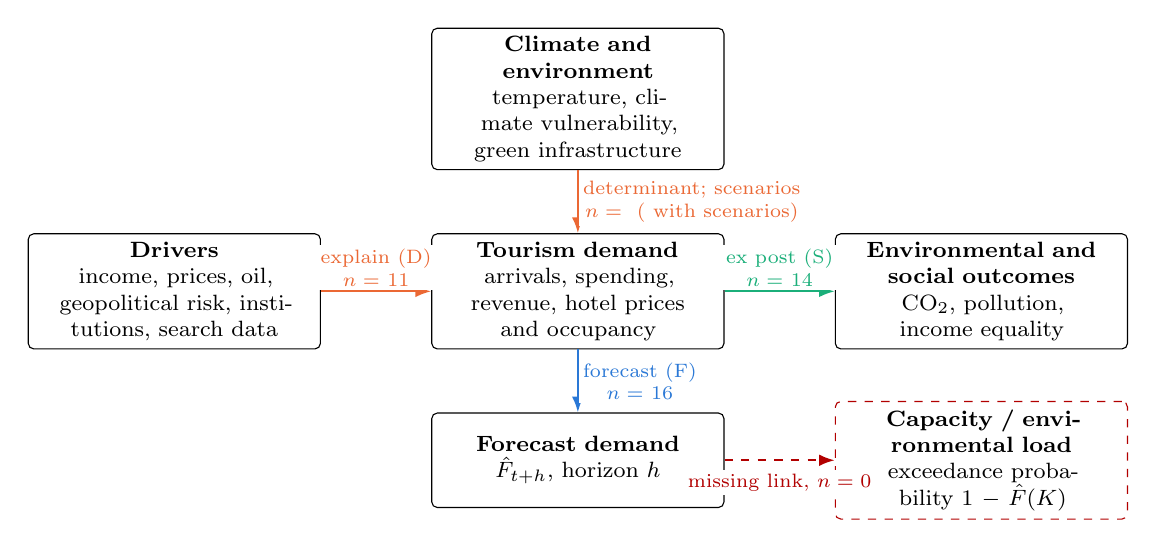
\begin{tikzpicture}[font=\footnotesize, node distance=8mm and 14mm,
  box/.style={draw, rounded corners=2pt, align=center, text width=3.5cm, minimum height=12mm, inner sep=3pt, fill=white},
  arr/.style={-{Latex[length=2mm]}, thick},
  lab/.style={font=\scriptsize, align=center, fill=white, inner sep=1.5pt}]
\definecolor{cF}{HTML}{2a78d6}\definecolor{cD}{HTML}{eb6834}\definecolor{cS}{HTML}{1baf7a}
\node[box] (drv) {\textbf{Drivers}\\ income, prices, oil, geopolitical risk, institutions, search data};
\node[box, right=of drv] (dem) {\textbf{Tourism demand}\\ arrivals, spending, revenue, hotel prices and occupancy};
\node[box, right=of dem] (env) {\textbf{Environmental and social outcomes}\\ CO$_2$, pollution, income equality};
\node[box, above=of dem] (cli) {\textbf{Climate and environment}\\ temperature, climate vulnerability, green infrastructure};
\node[box, below=of dem] (fc) {\textbf{Forecast demand}\\ $\hat F_{t+h}$, horizon $h$};
\node[box, right=of fc, dashed, draw=red!70!black] (cap) {\textbf{Capacity / environmental load}\\ exceedance probability $1-\hat F(K)$};
\draw[arr, cD] (drv) -- node[lab, above]{explain (D)\\ $n=$ \NnD{}} (dem);
\draw[arr, cS] (dem) -- node[lab, above]{ex post (S)\\ $n=$ \NnS{}} (env);
\draw[arr, cD] (cli) -- node[lab, right]{determinant; scenarios\\ $n=$ \NDenv{} (\NDscen{} with scenarios)} (dem);
\draw[arr, cF] (dem) -- node[lab, right]{forecast (F)\\ $n=$ \NnF{}} (fc);
\draw[arr, dashed, red!70!black] (fc) -- node[lab, below=3pt]{missing link, $n=0$} (cap);
\end{tikzpicture}

\caption{Framework of the tourism--environment links examined by the included studies. Solid arrows are links studied (number of studies); the dashed arrow is the missing link proposed for future research.}\label{fig:framework}
\end{figure}

\paragraph{Capacity-aware forecasting.}
We propose, as a \emph{hypothesised direction that has not been tested here}, that tourism forecasts for sustainability-sensitive destinations be evaluated not only by point accuracy but by the decision-relevant risk of exceeding capacity. Let $Y_{r,t+h}$ be visitors to region $r$ at horizon $h$, with predictive distribution $\hat F_{r,t+h}$ and environmental capacity $K_r$ (for example water, energy or site-carrying thresholds). The relevant quantity is the exceedance probability $\hat p_{r,t+h}=1-\hat F_{r,t+h}(K_r)$, assessed with proper scoring rules and calibration diagnostics. Such an agenda would require probabilistic forecasts, regionally disaggregated data and environmental indicators, none of which is combined in the included studies. The Saudi giga-project and heritage destinations make this question concrete, but testing it requires data not examined in this review. This agenda is not new in its aim: carrying-capacity research already builds early-warning indicator systems and forecasts them, for example with neural networks \citep{Ye2020}, and \citet{Long2022} call for dynamic forecasting of carrying capacity. The difference we propose is to derive warnings from probabilistic \emph{demand} forecasts, evaluated for calibration, rather than to forecast a composite warning index. Whether this improves decisions is an empirical question.

\subsection{Practical Implications}
For researchers: report accuracy metrics, benchmarks and forecast horizons in abstracts, and compare forecasts using accepted predictive-accuracy tests \citep{Diebold1995}. For policy: forecasts used for Vision 2030 planning should be accompanied by environmental-capacity analysis; the existing nexus studies report tourism--emissions links in GCC and UAE data, with signs that differ across tourism indicators and sustainability pillars \citep{Farooq2023a,Zmami2024,Majumdar2022}.


\subsection{Future Research Agenda}
Table~\ref{tab:agenda} lists research directions that follow from the gaps identified, each linked to the evidence in this review.

\begin{table}[t]\centering\small
\caption{Future lines of research.}\label{tab:agenda}
\begin{tabularx}{\linewidth}{@{}p{4.2cm}X@{}}
\toprule
Research line & Rationale from this review\\
\midrule
Probabilistic forecasts and prediction intervals & No forecasting abstract names prediction intervals or probabilistic forecasts (Section~\ref{sec:split}).\\
Capacity-aware evaluation of demand forecasts & No study links forecast demand to environmental load or capacity (Figure~\ref{fig:framework}); early-warning research forecasts indices instead \citep{Ye2020,Long2022}.\\
Forecast-based emission projections & Sustainability studies estimate tourism--emission elasticities ex post (\NnS{} studies) but none projects emissions from forecast arrivals.\\
Saudi regional and event-based forecasting & Only \NsaudiF{} Saudi forecasting studies; regional spending varies strongly across 13 regions \citep{Alfehaid2026}; religious tourism has distinct dynamics \citep{Mabrouk2026}.\\
Evaluation standards & Accuracy measures appear in only \NFmetric{} of \NFabs{} assessable abstracts (Figure~\ref{fig:measures}); benchmark and test reporting \citep{Hyndman2021fpp,Diebold1995}.\\
Search and big data & Only 3 of \NnF{} forecasting studies use search data, against a global trend \citep{Wu2024}.\\
\bottomrule
\end{tabularx}
\end{table}

\section{Conclusions}
\subsection{Limitations}\label{sec:limits}
\begin{enumerate}
\item \textbf{No full-text assessment.} The execution environment blocked publisher and DOI-resolver hosts, so all eligibility decisions and data extraction rest on Crossref metadata and abstracts. \Nnnoabs{} included records had no abstract. Extracted items marked n/r were never inferred.
\item \textbf{Single database, capped retrieval.} Crossref only; each query returned at most 100 records, although every query had more matches. Scopus, Web of Science, IEEE Xplore, Arabic-language and regional databases and grey literature were not searched.
\item \textbf{Imperfect automated screening.} A recall check against \Nother{} supplementary records found that two had been retrieved but removed by the automated filters and four had not been retrieved at all. The pipeline therefore missed relevant studies; a point estimate of pipeline recall over included studies is $37/42\approx 88\%$, which is an upper bound because the check was seeded from the same search family.
\item \textbf{Single reviewer.} The AI agent performed screening and coding with no independent human duplicate; no inter-rater reliability could be computed.
\item \textbf{No formal risk of bias, reporting-bias or certainty assessment} (PRISMA items 11, 14, 15, 18, 21, 22), and no effect-size pooling.
\item \textbf{Scope choices.} The definition of Middle East includes T\"urkiye and Iran; the exclusion of growth-only nexus studies is a judgement; the corpus includes economic-growth-adjacent sustainability outcomes only where an environmental, social or sustainability dimension was stated.
\item \textbf{Keyword-based sustainability coding} reflects abstract wording and may overlook relevant content.
\end{enumerate}
Because of limitations 1--4, the review should be read as a systematic mapping of a retrievable subset of the literature, and the paper requires full-text verification and, ideally, a second reviewer before submission to a journal.

\subsection{Contributions}
The review contributes a joint map of forecasting and sustainability evidence for Saudi Arabia and the Middle East, a quantified forecasting--sustainability split supported by both thematic coding and keyword co-occurrence, a framework of link directions, and a research agenda positioned against prior reviews and early-warning research.

\subsection{Concluding Remarks}

Within the retrievable Middle Eastern literature (\Nincluded{} studies), tourism forecasting and tourism-sustainability analysis are largely separate: forecasting studies seldom include sustainability and sustainability studies rarely project forward. Saudi Arabia has a growing but thin forecasting base. A capacity-aware, probabilistic forecasting agenda could connect the two. Verification against full texts, a second reviewer and additional databases are the necessary next steps.

\section*{Declarations}
\noindent\textbf{Registration and protocol:} not registered (see Methods). \textbf{Funding:} none declared \tbd. \textbf{Competing interests:} none declared \tbd. \textbf{AI assistance disclosure:} the search code, screening, data coding and drafting were performed by an AI agent (Claude Code), supervised by the author; the human author must verify all claims and citations before submission. \textbf{Data and code availability:} all search logs, screening outputs, coded data and scripts are in the repository directory \texttt{review/} (branch \texttt{claude/quirky-goldberg-12lm00}); records can be regenerated by running \texttt{search/crossref\_search.py}, \texttt{screen.py}, \texttt{screen\_stage2.py}, \texttt{build\_dataset.py} and \texttt{gen\_tex.py}.

\bibliographystyle{plainnat}
\bibliography{refs}

\appendix
\section{PRISMA 2020 checklist with item status}
\small
\begin{longtable}{@{}p{1.1cm}p{5.2cm}p{2.0cm}p{6.5cm}@{}}
\toprule
Item & Topic & Status & Where / comment\\
\midrule\endhead
1 & Title & Reported & Title identifies a systematic review.\\
2 & Abstract & Reported & Structured; PRISMA~2020 for Abstracts elements.\\
3 & Rationale & Reported & Sections 1--2.\\
4 & Objectives & Reported & RQ1--RQ4, Section 1.\\
5 & Eligibility criteria & Reported & Section 3.4, Table~\ref{tab:criteria}.\\
6 & Information sources & Partial & Crossref only; date stated (Section 3.2).\\
7 & Search strategy & Reported & Section 3.3, Table~\ref{tab:strings}, Appendix C; PRISMA-S not fully met.\\
8 & Selection process & Partial & Single AI reviewer; no duplicate (Section 3.5).\\
9 & Data collection process & Partial & Single reviewer, abstract-level (Section 3.6).\\
10a/b & Data items & Reported & Section 3.6, Table~\ref{tab:extraction}.\\
11 & Study risk of bias assessment & Partial/Not done & Reporting-transparency screen only (Section 3.7).\\
12 & Effect measures & Not applicable & No pooling.\\
13a--f & Synthesis methods & Reported & Descriptive, keyword and thematic analysis (Section 3.8).\\
14 & Reporting bias assessment & Not done & --\\
15 & Certainty assessment & Not done & --\\
16a/b & Study selection & Reported & Figure~\ref{fig:prisma}, Section 4.1, Appendix E.\\
17 & Study characteristics & Reported & Figures~\ref{fig:trend}--\ref{fig:settings}, Tables~\ref{tab:forecast}--\ref{tab:other}.\\
18 & Risk of bias in studies & Partial & Section 4.6.\\
19 & Results of individual studies & Partial & Abstract-level only.\\
20a--d & Results of syntheses & Partial & Sections 4.2--4.5; no meta-analysis.\\
21 & Reporting biases & Not done & --\\
22 & Certainty of evidence & Not done & --\\
23a--d & Discussion & Reported & Sections 5--6.\\
24a--c & Registration and protocol & Not done & Not registered.\\
25 & Support & Reported & None declared \tbd.\\
26 & Competing interests & Reported & None declared \tbd.\\
27 & Availability of data/code & Reported & Repository \texttt{review/}.\\
\bottomrule
\end{longtable}

\normalsize
\section{Coding scheme}
Theme: F, D or S (Section 3.4). Method family: C (classical statistical or econometric), M (machine or deep learning), H (hybrid, ensemble or multi-family comparison, e.g.\ classical versus neural models), G (grey). Benchmark: abstract names a comparison of models or benchmarks (y), none (n), unknown (n/r). Forward projection: a forecast beyond the sample or scenarios stated in the abstract. Sustainability: stated dimension; ``framing'' denotes the word ``sustainable'' used without a sustainability variable.

\section{Search log}\small
\begin{longtable}{@{}p{9.2cm}rr@{}}
\toprule
Query (\texttt{query.bibliographic}) & Reported total & Retrieved\\
\midrule\endhead
tourism demand forecasting Saudi Arabia & 412,893 & 100 \\
tourist arrivals forecasting Saudi Arabia & 206,248 & 100 \\
tourism forecasting machine learning Saudi Arabia & 1,685,238 & 100 \\
tourism forecasting deep learning Saudi Arabia & 1,771,597 & 100 \\
hotel occupancy forecasting Saudi Arabia & 218,316 & 100 \\
tourism sustainability prediction Saudi Arabia & 894,148 & 100 \\
tourism CO2 emissions Saudi Arabia & 423,634 & 100 \\
sustainable tourism modelling Saudi Arabia & 884,515 & 100 \\
tourism demand forecasting Middle East & 630,664 & 100 \\
tourist arrivals forecasting Middle East & 424,968 & 100 \\
tourism forecasting machine learning Middle East & 1,899,471 & 100 \\
tourism forecasting deep learning Middle East & 1,985,114 & 100 \\
hotel occupancy forecasting Middle East & 437,099 & 100 \\
tourism sustainability prediction Middle East & 1,111,210 & 100 \\
tourism CO2 emissions Middle East & 641,367 & 100 \\
sustainable tourism modelling Middle East & 1,101,189 & 100 \\
tourism demand forecasting GCC & 319,454 & 100 \\
tourist arrivals forecasting GCC & 112,281 & 100 \\
tourism forecasting machine learning GCC & 1,594,056 & 100 \\
tourism forecasting deep learning GCC & 1,680,493 & 100 \\
hotel occupancy forecasting GCC & 124,380 & 100 \\
tourism sustainability prediction GCC & 801,859 & 100 \\
tourism CO2 emissions GCC & 330,019 & 100 \\
sustainable tourism modelling GCC & 792,073 & 100 \\
tourism demand forecasting Hajj Umrah & 323,426 & 100 \\
tourist arrivals forecasting Hajj Umrah & 116,271 & 100 \\
tourism forecasting machine learning Hajj Umrah & 1,597,894 & 100 \\
tourism forecasting deep learning Hajj Umrah & 1,684,325 & 100 \\
hotel occupancy forecasting Hajj Umrah & 128,367 & 100 \\
tourism sustainability prediction Hajj Umrah & 805,908 & 100 \\
tourism CO2 emissions Hajj Umrah & 334,023 & 100 \\
sustainable tourism modelling Hajj Umrah & 796,103 & 100 \\
tourism demand forecasting Gulf Cooperation Council & 426,549 & 100 \\
tourism sustainability Gulf Cooperation Council & 553,013 & 100 \\
tourism demand forecasting GCC & 319,454 & 100 \\
tourism sustainability GCC & 446,420 & 100 \\
tourism demand forecasting Middle East & 630,664 & 100 \\
tourism sustainability Middle East & 756,893 & 100 \\
tourism demand forecasting MENA & 331,865 & 100 \\
tourism sustainability MENA & 458,825 & 100 \\
tourism demand forecasting Dubai & 320,131 & 100 \\
tourism sustainability Dubai & 447,184 & 100 \\
tourism demand forecasting UAE & 323,571 & 100 \\
tourism sustainability UAE & 450,488 & 100 \\
tourism demand forecasting United Arab Emirates & 549,400 & 100 \\
tourism sustainability United Arab Emirates & 675,840 & 100 \\
tourism demand forecasting Qatar & 323,738 & 100 \\
tourism sustainability Qatar & 450,720 & 100 \\
tourism demand forecasting Oman & 328,493 & 100 \\
tourism sustainability Oman & 455,487 & 100 \\
tourism demand forecasting Bahrain & 319,661 & 100 \\
tourism sustainability Bahrain & 446,731 & 100 \\
tourism demand forecasting Kuwait & 323,597 & 100 \\
tourism sustainability Kuwait & 450,655 & 100 \\
tourism demand forecasting Jordan & 362,023 & 100 \\
tourism sustainability Jordan & 488,890 & 100 \\
tourism demand forecasting Egypt & 388,672 & 100 \\
tourism sustainability Egypt & 515,428 & 100 \\
tourism demand forecasting Turkey & 382,632 & 100 \\
tourism sustainability Turkey & 509,550 & 100 \\
tourism demand forecasting Iran & 426,257 & 100 \\
tourism sustainability Iran & 553,094 & 100 \\
tourism demand forecasting Morocco & 336,617 & 100 \\
tourism sustainability Morocco & 463,578 & 100 \\
tourism demand forecasting Tunisia & 326,643 & 100 \\
tourism sustainability Tunisia & 453,654 & 100 \\
tourism demand forecasting Lebanon & 323,843 & 100 \\
tourism sustainability Lebanon & 450,895 & 100 \\
tourism demand forecasting Israel & 351,835 & 100 \\
tourism sustainability Israel & 478,874 & 100 \\
\bottomrule
\end{longtable}


\normalsize
\section{Records and code}
Raw Crossref records (\texttt{data/crossref\_raw.json}), the log (\texttt{data/search\_log.json}), screening outputs, the coded dataset (\texttt{data/included.json}), and the PRISMA counts (\texttt{data/final\_numbers.json}) are in the repository. Web-search leads from the earlier screening passes are in \texttt{data/stream*.json}; they are unverified and were used only to seed the targeted searches.

\section{Records excluded at eligibility assessment}\scriptsize
\begin{longtable}{@{}p{3.6cm}p{7.3cm}p{0.8cm}p{3.4cm}@{}}
\toprule
DOI & Title (truncated) & Year & Reason\\
\midrule\endhead
10.52133/ijrsp.v6.71.6 & Enhancing Risk Management in Events by Providing AI-Risk Assessment Framework & 2025 & Not quantitative forecast/demand/sustainability study \\
10.18089/tms.2022.180302 & Effect of internal corporate social responsibility activities on tourism and hospitality employ & 2022 & Not quantitative forecast/demand/sustainability study \\
10.30892/gtg.634spl28-1643 & THE TRANSFORMATIVE ROLE OF PLACE ATTACHMENT IN CONVERTING SUSTAINABILITY PERCEPTIONS INTO ACTIV & 2025 & Not quantitative forecast/demand/sustainability study \\
10.3727/108354215x14464845877995 & Religious Tourism and Economic Growth in Oil-Rich Countries: Evidence from Saudi Arabia & 2015 & Growth nexus only \\
10.18488/31.v12i2.4595 & Hybrid tourism and territorial development: The case of voluntourism and alternative tourism in & 2025 & Not quantitative forecast/demand/sustainability study \\
10.34021/ve.2020.03.04(2) & The Relation between Tourism and Economic Growth: A Case of Saudi Arabia as an Emerging Tourism & 2020 & Growth nexus only \\
10.3390/economies9030117 & The Role of Tourism in Economic Growth: Empirical Evidence from Saudi Arabia & 2021 & Growth nexus only \\
10.21833/ijaas.2021.09.008 & COVID-19 and tourism sector: A perspective of Saudi Arabia & 2021 & Not quantitative forecast/demand/sustainability study \\
10.30892/gtg.662spl37-1798 & THE INFLUENCE OF THE DIVERSITY OF TOURIST REGIONS ON THE CHOICE OF TOURIST DESTINATIONS IN SAUD & 2026 & Not quantitative forecast/demand/sustainability study \\
10.3390/su132313372 & Forecasting the Impact of Gross Domestic Product (GDP) on International Tourist Arrivals to Lan & 2021 & Outside Middle East \\
10.30519/ahtr.990903 & Forecasting Tourist Arrivals to Sangiran Using Fuzzy with Calendar Variations & 2022 & Outside Middle East \\
10.1108/jhti-03-2024-0223 & Enabling hotel circularity via Industry 4.0 innovations for enhanced hotel performance: insight & 2024 & Not quantitative forecast/demand/sustainability study \\
10.3390/su17052328 & Leveraging Spectral Clustering and Long Short-Term Memory Techniques for Green Hotel Recommenda & 2025 & Not quantitative forecast/demand/sustainability study \\
10.30892/gtg.43321-915 & THE IMPACT OF RELIGIOUS TOURISTS’ SATISFACTION WITH HAJJ SERVICES ON THEIR EXPERIENCE AT THE SA & 2022 & Not quantitative forecast/demand/sustainability study \\
10.3390/su18063124 & Sustainable Destination Marketing in Saudi Arabia: Effects of Sustainability Storytelling and S & 2026 & Not quantitative forecast/demand/sustainability study \\
10.55908/sdgs.v11i11.1639 & Challenges Facing Tourism for People with Disabilities (Accessible Tourism) in the Kingdom of S & 2023 & Not quantitative forecast/demand/sustainability study \\
10.24922/eot.v6i2.53474 & Motivation towards Inbound Tourism: A Study of Middle East Tourist & 2019 & Not quantitative forecast/demand/sustainability study \\
10.63556/jotags.2026.1930 & Türkiye'ye Yönelik Yabancı Turizm Talebinin Öngörülmesi: Reel Efektif Döviz Kuru, Mevsimsellik  & 2026 & Non-English / proceedings \\
10.14505/jemt.v14.4(68).03 & The Contribution of Tourism Industry Cash Flows to Economic Growth “Middle East Evidence” & 2023 & Growth nexus only \\
10.24114/cess.v7i2.33959 & Forecasting Room Occupancy Rates Based on Hotel Class in Bali Using the ARIMA Method & 2022 & Outside Middle East \\
10.3390/su12229620 & Urban Sprawl, Socioeconomic Features, and Travel Patterns in Middle East Countries: A Case Stud & 2020 & Not quantitative forecast/demand/sustainability study \\
10.32479/ijeep.14410 & Do Tourism and Renewable Energy Influence CO2 Emissions in Tourism-Dependent Countries? & 2023 & Region/tourism link unconfirmed \\
10.1371/journal.pone.0328456 & Estimating CO2 emissions due to present and future suborbital space tourism industry & 2025 & Outside Middle East \\
10.3390/su8070605 & Is Tourism Development a Sustainable Economic Growth Strategy in the Long Run? Evidence from GC & 2016 & Growth nexus only \\
10.3390/su162310760 & Transport Sector Emissions and Environmental Sustainability: Empirical Evidence from GCC Econom & 2024 & Region/tourism link unconfirmed \\
10.3390/su17115058 & Sustainable Tourism and Its Environmental and Economic Impacts: Fresh Evidence from Major Touri & 2025 & Outside Middle East \\
10.29313/amwaluna.v8i1.3476 & Bibliometric Analysis of Halal Tourism (Hajj and Umrah) Development in the World & 2024 & Not quantitative forecast/demand/sustainability study \\
10.47747/ijmhrr.v5i2.1705 & The Influence of Service Quality, Prices, and Promotions on the Satisfaction of Pilgrims on Haj & 2024 & Not quantitative forecast/demand/sustainability study \\
10.55677/gjefr/02-2025-vol02e10 & Shariah-Compliant Financial Services for Hajj and Umrah: Products, Challenges, and Policy Recom & 2025 & Not quantitative forecast/demand/sustainability study \\
10.1109/access.2025.3532385 & Machine Learning-Integrated Usability Evaluation and Monitoring of Human Activities for Individ & 2025 & Operational/crowd/health prediction \\
10.1016/j.aej.2025.12.032 & Predictive analysis of Hajj and Umrah performance using key performance indicators (KPIs) and m & 2026 & Operational/crowd/health prediction \\
10.61132/wjilt.v2i3.434 & Digital Books as Learning Media for Islamic Religious Education on Hajj and Umrah Material for  & 2025 & Not quantitative forecast/demand/sustainability study \\
10.1016/j.eswa.2023.122204 & A customized deep learning-based framework for classification and analysis of social media post & 2024 & Not quantitative forecast/demand/sustainability study \\
10.21580/nw.2025.19.1.26704 & Building Virtual Reality Hajj Journey Learning Media  as a Simulation Tool for Teaching Hajj an & 2025 & Not quantitative forecast/demand/sustainability study \\
10.38035/jgia.v3i4.568 & Economic Improvement Based on Hajj and Umrah Business in Indonesia & 2025 & Not quantitative forecast/demand/sustainability study \\
10.1109/access.2024.3394905 & Crowd Congestion Forecasting Framework Using Ensemble Learning Model and Decision Making Algori & 2024 & Operational/crowd/health prediction \\
10.5339/jist.2025.12 & Utilizing information technology to address challenges in Hajj and Umrah: A narrative review & 2025 & Not quantitative forecast/demand/sustainability study \\
10.55041/ijsrem37043 & 3D Modelling for the Hajj and Umrah Pilgrims & 2024 & Not quantitative forecast/demand/sustainability study \\
10.1016/j.aej.2025.06.043 & Smart mobile application for real-time monitoring and prediction of pilgrim crowd activities in & 2025 & Operational/crowd/health prediction \\
10.24191/idealogy.v10i2.834 & An Analysis on 3D Modelling Technique in Virtual Reality for Hajj and Umrah Simulation & 2025 & Not quantitative forecast/demand/sustainability study \\
10.1080/1528008x.2025.2599751 & A PLS – Neural Network Approach to Study Factors Influencing Gulf Cooperation Council Tourists’ & 2025 & Not quantitative forecast/demand/sustainability study \\
10.53596/ma0frs79 & Regional Tourism and Global Challenges in the Face of Political Uncertainty: Case STUDY of the  & 2025 & Not quantitative forecast/demand/sustainability study \\
10.14505//jemt.v12.2(50).29 & The Contribution of Tourism to Economic Growth: The Case of Qatar & 2021 & Growth nexus only \\
10.47259/ijrebs.2025.634 & Revitalization of Oman’s Tourism Destinations through the Omani Youth’s Level of Engagement and & 2025 & Not quantitative forecast/demand/sustainability study \\
10.3727/154427320x15828792518754 & An Analytical Approach to Cruise Tourism As an Option For Development: a Case Study of the Sult & 2020 & Not quantitative forecast/demand/sustainability study \\
10.3390/admsci12040168 & Fusion of Sustainability in the Tourism Industry for Improved Competitiveness: Investigation of & 2022 & Not quantitative forecast/demand/sustainability study \\
10.3390/su11071907 & Residents’ Perceptions and Satisfaction toward Tourism Development: A Case Study of Petra Regio & 2019 & Not quantitative forecast/demand/sustainability study \\
10.30892/gtg.50403-1121 & PERCEPTION OF LOCAL COMMUNITY TOWARDS TOURISM DEVELOPMENT: A STUDY ON RURAL TOURISM SITES OF JO & 2023 & Not quantitative forecast/demand/sustainability study \\
10.30892/gtg.58105-1390 & TOURISM EXPERIENCES, MOTIVATIONS, AND TRAVEL LIFESTYLES PREFERENCES FOR DOMESTIC TOURISTS: A CA & 2025 & Not quantitative forecast/demand/sustainability study \\
10.3390/su151310013 & Determinants of Residents’ Support for Sustainable Tourism Development: An Empirical Study in M & 2023 & Not quantitative forecast/demand/sustainability study \\
10.18092/ulikidince.442734 & RELIGION AND TOURISM IN TURKEY: AN ECONOMICALLY EMPIRICAL STUDY RELIGION AND TOURISM IN TURKEY: & 2019 & Growth nexus only \\
10.31201/ijhmt.696185 & AGRO TOURISM IN TURKEY & 2020 & Not quantitative forecast/demand/sustainability study \\
10.34190/eckm.27.1.4788 & Hybrid ARIMA-LSTM Knowledge Management for Strategic Tourism Demand Forecasting in Morocco & 2026 & Non-English / proceedings \\
10.55677/gjefr/10-2024-vol01e7 & VECM Model Analysis of the Causality between Tourism, Foreign Direct Investment and Economic Gr & 2024 & Growth nexus only \\
10.1177/1354816619836338 & Tourism–growth nexus under duress: Lebanon during the Syrian crisis & 2019 & Growth nexus only \\
10.1016/j.ijhm.2026.104745 & Hybrid machine learning approaches for hotel occupancy forecasting: Evaluating gradient boostin & 2026 & Region/tourism link unconfirmed \\
\bottomrule
\end{longtable}

\end{document}
